\documentclass[11pt,letterpaper]{report}
\usepackage{amssymb,amsfonts,color,graphicx,amsmath,enumerate}
\usepackage{amsthm}

\newcommand{\naturals}{\mathbb{N}}
\newcommand{\integers}{\mathbb{Z}}
\newcommand{\complex}{\mathbb{C}}
\newcommand{\reals}{\mathbb{R}}
\newcommand{\mcal}[1]{\mathcal{#1}}
\newcommand{\rationals}{\mathbb{Q}}
\newcommand{\field}{\mathbb{F}}
\newcommand{\Var}{\text{Var}}
\newcommand{\ind}{\mathbbm{1}}
\newcommand{\Cov}{\text{Cov}}

\newenvironment{solution}
{\begin{proof}[Solution]}
{\end{proof}}

\voffset=-3cm
\hoffset=-2.25cm
\textheight=24cm
\textwidth=17.25cm
\addtolength{\jot}{8pt}
\linespread{1.3}

\begin{document}
\begin{center}
{\bf \Large Math 130B - Conditional Expectation}
\vspace{0.2cm}
\hrule
\end{center}
\begin{enumerate}
	%https://www.stat.auckland.ac.nz/~fewster/325/notes/ch3.pdf
	\item A mouse is placed in a maze with two rooms pictured in Figure 1. Starting from room 1, what is the expected number of steps the mouse takes before it reaches the exit?
	\begin{figure}[h]
		\centering
			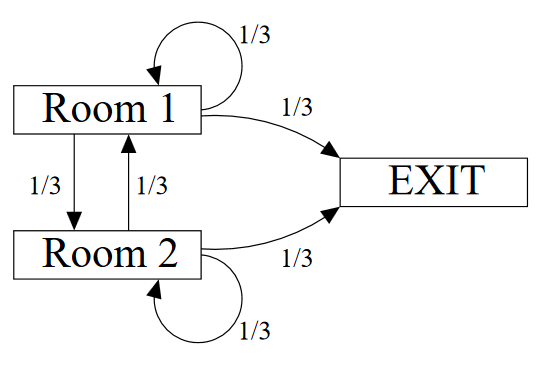
\includegraphics[scale=.6]{diagram.PNG}
			\caption{Maze}
	\end{figure}
	\vfill
	%https://people.eecs.berkeley.edu/~wlr/226F06/HW/problem-set2-sol.pdf
	\item On the day before an exam, Math 130B students go to Liam's office hours to ask questions. Each question asked will appear on the exam with probability $p$. The number of questions asked is a Poisson distributed random variable with mean $\lambda$. What is the probability that Liam does not have to answer an exam question?

	\vfill

	%https://www2.isye.gatech.edu/~sman/courses/6761/6761-2-ConditionalExpectation.pdf
	\item If $X$ and $Y$ are independent continuous random variables, show that
	\[
	\Pr[Y<X] = \int_\reals F_Y(x)f_X(x)\ dx,
	\]
	where $F_Y(\cdot)$ is the cdf of $Y$ and $f_X(\cdot)$ is the pdf of $X$. Use this to compute $\Pr[Y<X]$ where $X\sim Exp(\mu)$ and $Y\sim Exp(\lambda)$ are independent.
	\vfill
\end{enumerate}


\end{document}